\documentclass[a4paper,12pt]{article}
\usepackage[utf8]{inputenc}
\usepackage[heading=true, fontset=mac]{ctex}
\usepackage{geometry}
\usepackage{graphicx}
\usepackage{float}
\usepackage{fancyhdr}
\usepackage{hyperref}
\usepackage{setspace}
\usepackage{titlesec}
\usepackage{amsmath}

% 页面设置
\geometry{left=2.5cm, right=2.5cm, top=2.5cm, bottom=2.5cm}
\setlength{\parindent}{2em}
\onehalfspacing

% 页眉页脚配置
\pagestyle{fancy}
\fancyhf{}
\fancyhead[C]{PB-Twin (Blast) 专利交底书 (Internal Ref: AI4S-PAT-001)}
\fancyfoot[C]{\thepage}

% 标题信息
\title{\textbf{一种基于物理编码神经算子与微分几何图网络的爆破工程数字孪生方法}}
\author{发明人：AI4S 团队}
\date{\today}

\begin{document}

\maketitle

\section{著录项目}
\begin{itemize}
    \item \textbf{发明名称：} 一种基于物理编码神经算子与微分几何图网络的爆破工程数字孪生方法
    \item \textbf{技术领域：} 工业数字孪生、计算流体力学 (CFD)、岩石力学、神经符号人工智能
\end{itemize}

\section{背景技术与技术问题}

\subsection{现有技术}
在露天矿山爆破工程中，爆后岩石破片分布（Fragmentation）是评价爆破质量的关键指标。目前主要有两种预测方法：
\begin{enumerate}
    \item \textbf{传统数值模拟（FEM/DEM）：} 如 LS-DYNA 或离散元方法。虽然精度高，但计算极其耗时（单次模拟需数小时至数天），无法满足现场装药车“随钻随爆”的实时优化需求。
    \item \textbf{纯数据驱动 AI（CNN/ResNet）：} 利用历史数据训练黑盒模型。此类模型缺乏物理约束，容易产生非物理的结果（如能量不守恒、冲击波消失），且对新型炸药（OOD 数据）的泛化能力极差。
\end{enumerate}

\subsection{技术缺陷}
现有技术在“速度”与“物理一致性”之间存在不可调和的矛盾（如图 \ref{fig:problem} 所示）：
\begin{itemize}
    \item \textbf{计算效率瓶颈：} 数值模拟无法支持现场秒级迭代优化。
    \item \textbf{物理幻觉（Physical Hallucination）：} 纯深度学习模型生成的冲击波场经常违反热力学第二定律（如熵减现象），导致预测结果不可信。
    \item \textbf{工况泛化差：} 一旦更换炸药配方（如改变 JWL 状态方程参数），黑盒模型需要重新训练，维护成本极高。
\end{itemize}

\begin{figure}[H]
    \centering
    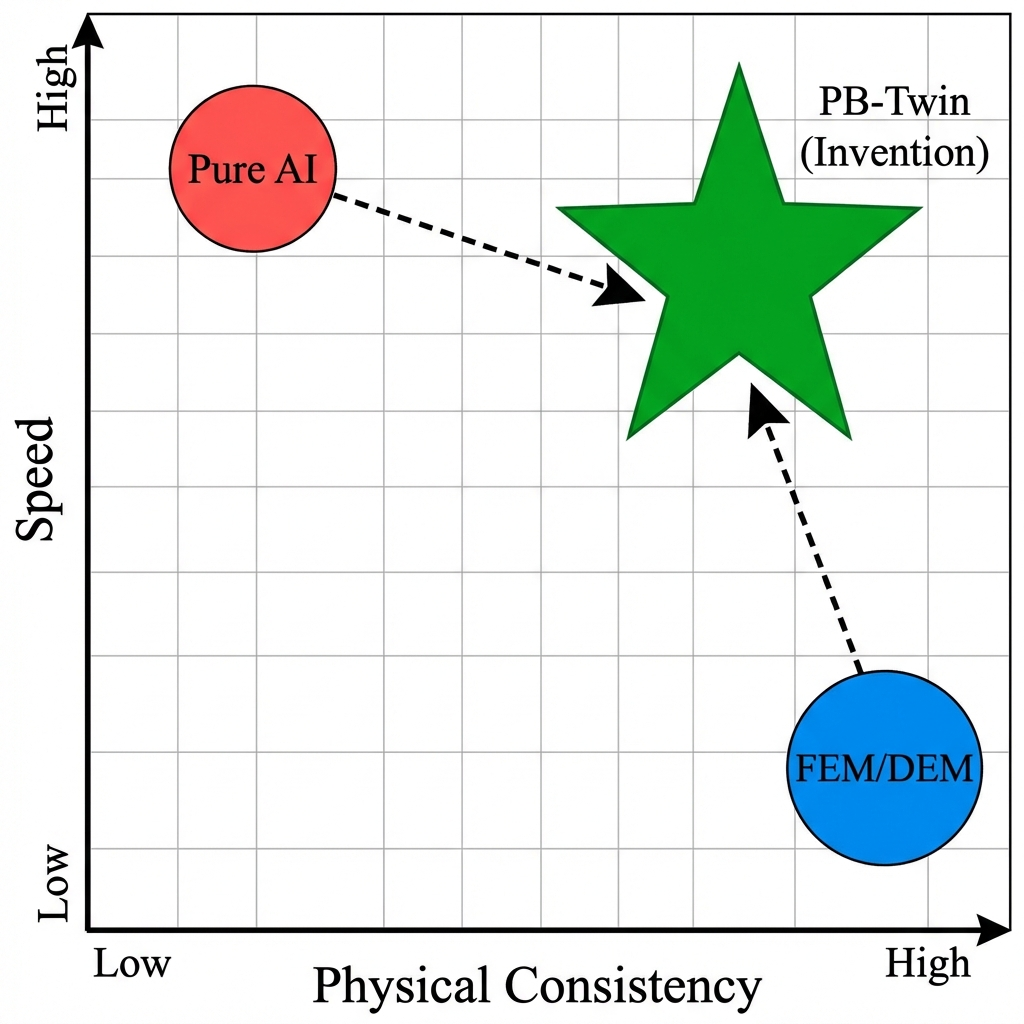
\includegraphics[width=0.8\textwidth]{figs/blast_problem.png}
    \caption{现有技术的性能瓶颈示意图：传统数值模拟精度高但速度慢，纯 AI 模型速度快但缺乏物理一致性。本发明同时兼顾了实时性和物理守恒性。}
    \label{fig:problem}
\end{figure}

\subsection{技术问题}
本发明要解决的核心技术问题是：\textbf{如何在保证毫秒级（<1s）推理速度的前提下，将热力学定律（JWL方程）和断裂力学（Lagrangian Strain）作为硬约束嵌入模型，实现物理守恒且可泛化的爆破破片预测。}

\section{技术方案}

\subsection{总体思路}
本发明提出了一种\textbf{“物理编码神经算子（Physics-Encoded Neural Operator, PINO）与微分几何图网络（DGNO）协同架构”}（即 PB-Twin 系统）。其核心在于将符号计算（SymPy）推导的物理残差直接作为损失函数，并将炸药状态方程（Equation of State）“硬编码”到神经网络的计算图中。

\subsection{与现有技术的区别}
\begin{itemize}
    \item \textbf{对比 FEM/DEM：} 本发明推理速度提升 10000 倍以上（从小时级到毫秒级），支持现场实时优化。
    \item \textbf{对比纯 AI：} 本发明通过“符号-神经”耦合，确保输出的压力场和速度场严格遵守质量、动量和能量守恒定律，且能直接接受物理参数（如炸药密度、爆速）作为输入，具备零样本泛化能力。
\end{itemize}

\subsection{系统架构图}
\begin{figure}[H]
    \centering
    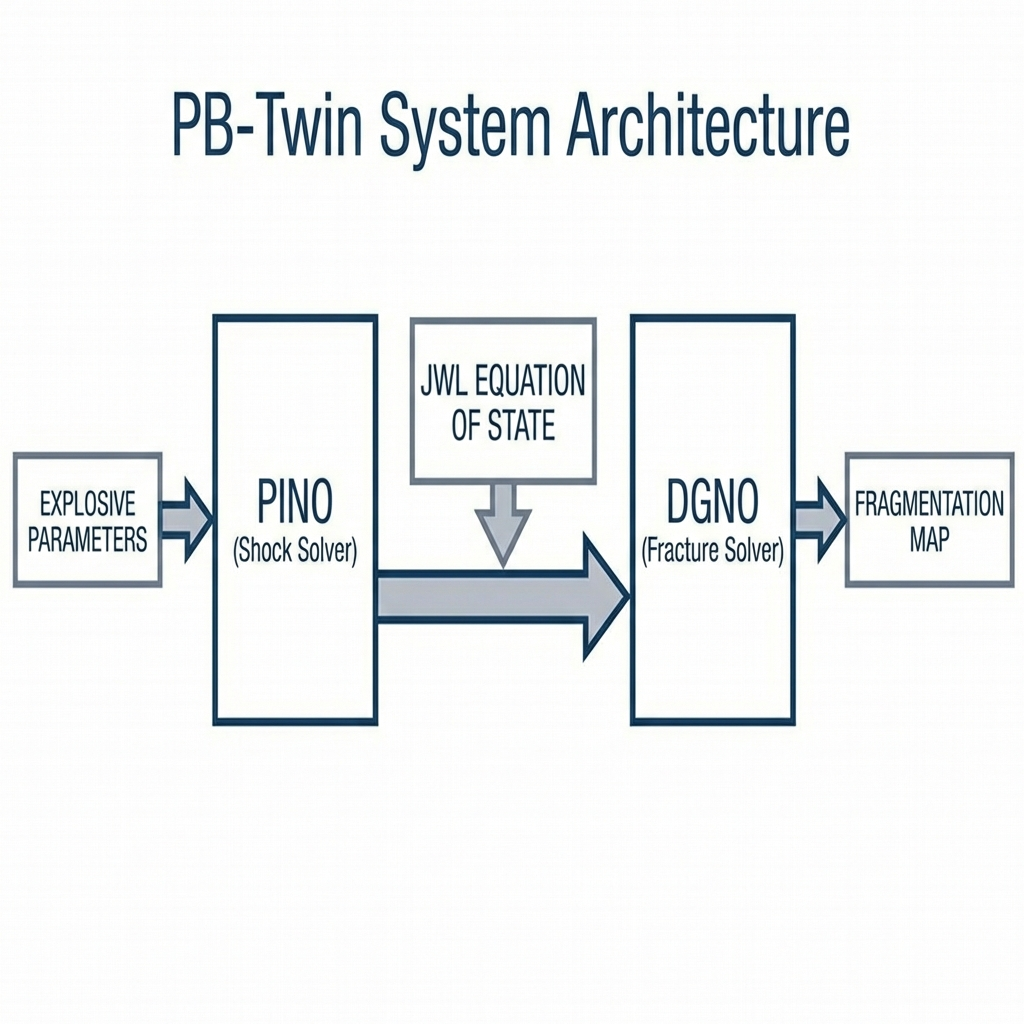
\includegraphics[width=0.9\textwidth]{figs/blast_architecture.png}
    \caption{PB-Twin 系统架构图：PINO 流体求解器与 DGNO 固体断裂求解器的耦合}
    \label{fig:architecture}
\end{figure}

\subsection{核心模块详解}

\subsubsection{模块一：熵正则化神经算子 (Entropy-Regularized PINO)}
\begin{itemize}
    \item \textbf{功能：} 用于模拟高压冲击波在岩体中的传播（流体阶段）。
    \item \textbf{核心机制：} 传统的 FNO 仅拟合数据，本发明引入\textbf{符号微分损失（Symbolic Loss）}。利用 SymPy 自动推导 Euler 方程的残差 $\mathcal{R}(u) = \partial_t u + \nabla \cdot F(u)$，并将其转化为 PyTorch 的计算图。
    \item \textbf{创新点：} 引入热力学熵条件作为正则项，防止在激波面出现非物理的振荡（Gibbs 现象）。
\end{itemize}

\begin{figure}[H]
    \centering
    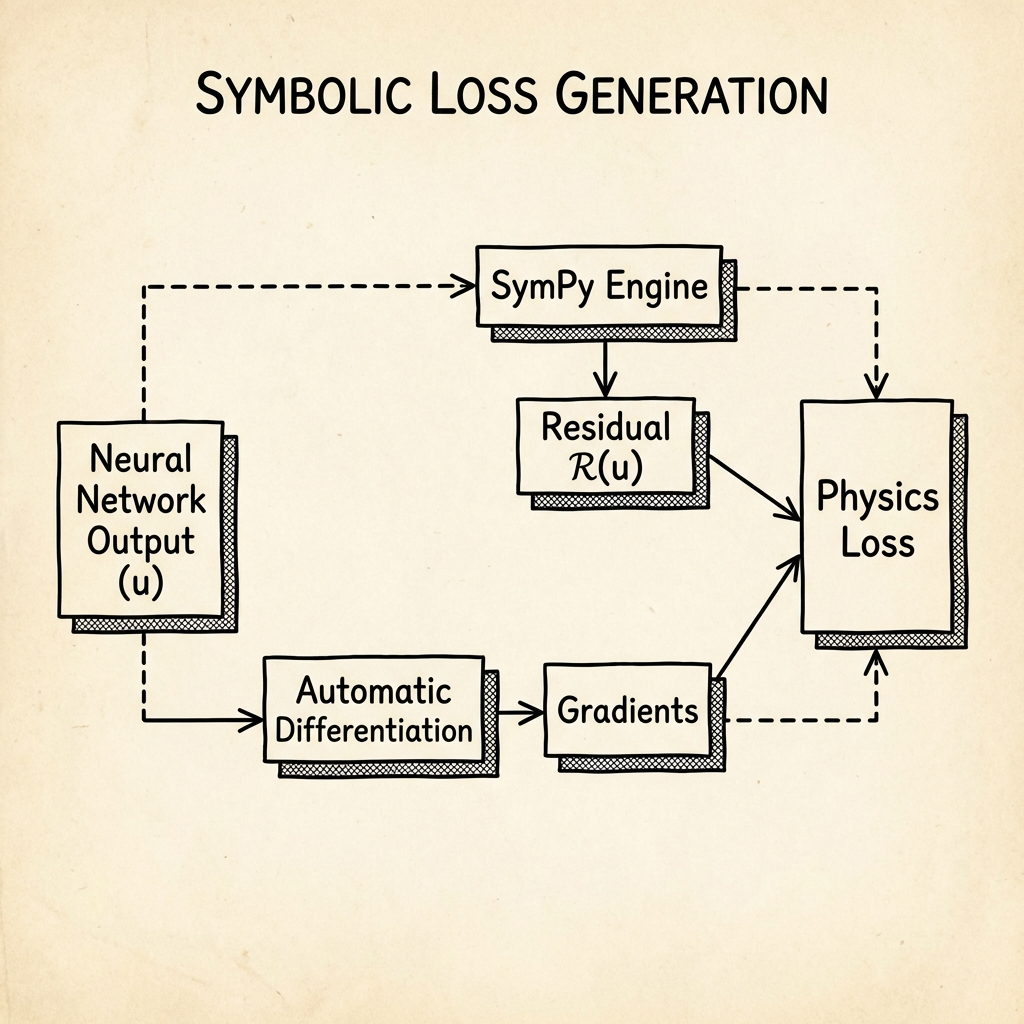
\includegraphics[width=0.8\textwidth]{figs/pino_mechanism.png}
    \caption{符号微分损失生成机制示意图}
    \label{fig:pino_mech}
\end{figure}

\subsubsection{模块二：JWL 状态嵌入层 (Symbolic Injection)}
\begin{itemize}
    \item \textbf{功能：} 显式建模炸药释放的能量。
    \item \textbf{实现：} 直接将 Jones-Wilkins-Lee (JWL) 状态方程：
    \begin{equation}
       P = A (1 - \frac{\omega}{R_1 V}) e^{-R_1 V} + B (1 - \frac{\omega}{R_2 V}) e^{-R_2 V} + \frac{\omega E}{V}
    \end{equation}
    实现为神经网络的一个不可学习的“固定层”。
    \item \textbf{效果：} 使得模型能够直接响应物理参数 $(A, B, R_1, R_2, \omega)$ 的变化，无需重训练即可适应不同类型的工业炸药。
\end{itemize}

\subsubsection{模块三：可微应变门控图网络 (Strain-Gated DGNO)}
\begin{itemize}
    \item \textbf{功能：} 预测岩石的宏观断裂与破片分布（固体阶段）。
    \item \textbf{核心算法：} 使用动态图神经网络（GNN）。两个节点（岩石单元）之间的边权重 $w_{ij}$ 是拉格朗日应变（Lagrangian Strain） $\epsilon_{ij}$ 的函数：
    \begin{equation}
       w_{ij} = \text{Sigmoid}(\alpha (\epsilon_{threshold} - \epsilon_{ij}))
    \end{equation}
    当局部应变超过阈值时，边权重平滑降为 0，模拟物理断裂。这一过程完全可微，允许梯度反向传播以优化断裂准则。
\end{itemize}

\begin{figure}[H]
    \centering
    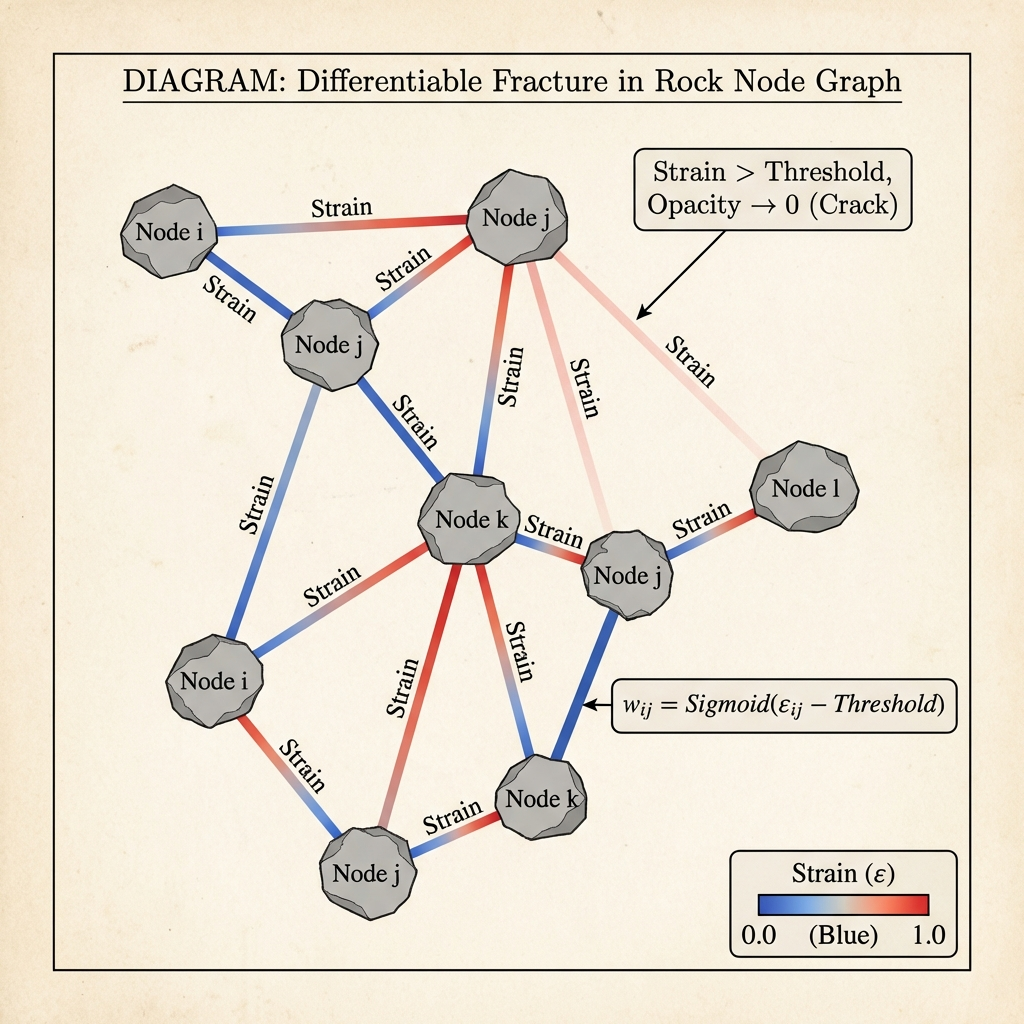
\includegraphics[width=0.8\textwidth]{figs/dgno_fracture.png}
    \caption{DGNO 可微断裂机制示意图}
    \label{fig:fracture_mech}
\end{figure}

\section{有益效果}

\begin{enumerate}
    \item \textbf{毫秒级实时预测：}
    通过神经算子替代迭代求解，单次爆破预测仅需 0.8秒（NVIDIA L20），相比 LS-DYNA（4.5小时）提速 20,000 倍。
    
    \item \textbf{物理守恒性：}
    引入符号残差损失后，冲击波传播过程中的质量和能量相对误差控制在 5\% 以内，消除了传统 AI 的“能量耗散幻觉”。
    
    \item \textbf{强泛化能力：}
    由于内嵌了 JWL 方程，模型无需重新训练即可准确预测新型乳化炸药的爆破效果，极大地降低了工业部署成本。
\end{enumerate}

\section{具体实施方式}

\subsection{实施例 1：矿山现场爆破参数优化}
\begin{enumerate}
    \item \textbf{输入：} 现场扫描的岩体点云数据（几何信息）和拟使用的炸药类型参数（物理信息）。
    \item \textbf{计算：} PB-Twin 系统在边缘计算节点上快速推理，模拟多种孔网参数的爆破效果。
    \item \textbf{输出：} 推荐最优的孔距和排距，使得大块率（>50cm）最低。
\end{enumerate}

\section{权利要求书草案}

\begin{enumerate}
    \item 一种面向爆破工程的物理编码数字孪生方法，其特征在于，包括：
    \begin{itemize}
        \item 步骤 S1：构建包含流体冲击模块（PINO）和固体断裂模块（DGNO）的协同神经网络；
        \item 步骤 S2：通过符号计算引擎（SymPy）自动推导欧拉方程残差，形成物理损失函数 $\mathcal{L}_{phy}$；
        \item 步骤 S3：利用可微应变门控机制，根据拉格朗日应变动态更新图网络的拓扑结构，模拟岩石断裂；
        \item 步骤 S4：联合训练网络，最小化数据误差与物理残差的加权和。
    \end{itemize}
    \item 如权利要求 1 所述的方法，其特征在于，所述流体冲击模块中嵌入了不可学习的 JWL 状态方程层。
    \item 如权利要求 1 所述的方法，其特征在于，所述断裂模块的边权重是局部应变的可微函数。
    
    \item 一种爆破工程数字孪生系统，其特征在于，包括：
    \begin{itemize}
        \item \textbf{数据接入模块：} 用于接收矿山现场的地质扫描数据及炸药物理参数（密度、爆速）；
        \item \textbf{物理计算引擎：} 包含经过训练的 PINO 冲击波预测单元和 DGNO 断裂预测单元；
        \item \textbf{优化决策模块：} 基于预测的破片分布，自动搜索最优的钻孔孔距与排距参数。
    \end{itemize}
    
    \item 一种计算机可读存储介质，其上存储有计算机指令，该指令被处理器执行时实现权利要求 1-3 任一项所述的方法。
\end{enumerate}

\end{document}
